\chapter{Optimization Algorithms}
如果梯度只用来指示方向,大小完全由lr决定?
\section{Challenges}

\begin{figure}
    \centering
    \begin{minipage}[b]{0.32\textwidth}
        \centering
        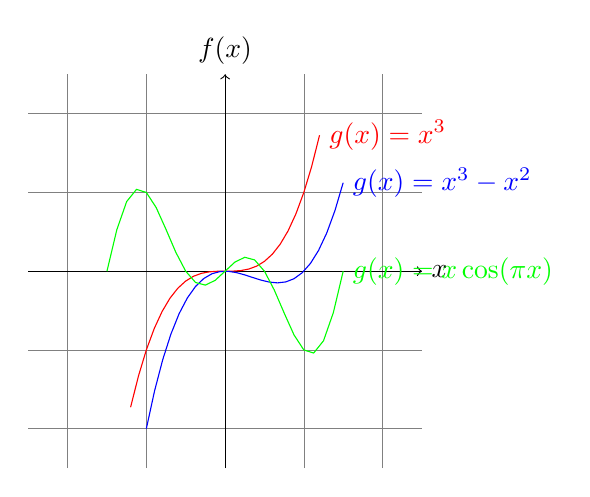
\begin{tikzpicture}
            \draw[very thin,color=gray] (-2.5, -2.5) grid (2.5, 2.5);
            \draw[->] (-2.5,0) -- (2.5,0) node[right] {$x$};
            \draw[->] (0,-2.5) -- (0,2.5) node[above] {$f(x)$};
            \draw[red,domain=-1.2:1.2]	plot (\x, { \x * \x * \x })   	node[right] {$g(x) = x^3 $};
            \draw[blue,domain=-1.0:1.5]	plot (\x, { \x * \x * \x - \x * \x })   	node[right] {$g(x) = x^3 - x^2$};
            \draw[green,domain=-1.5:1.5]	plot (\x, { \x * cos(3.1415926 * \x r) })   	node[right] {$g(x) = x\cos(\pi x) $};
        \end{tikzpicture}
    \end{minipage}
    \begin{minipage}[b]{0.32\textwidth}
        \centering
        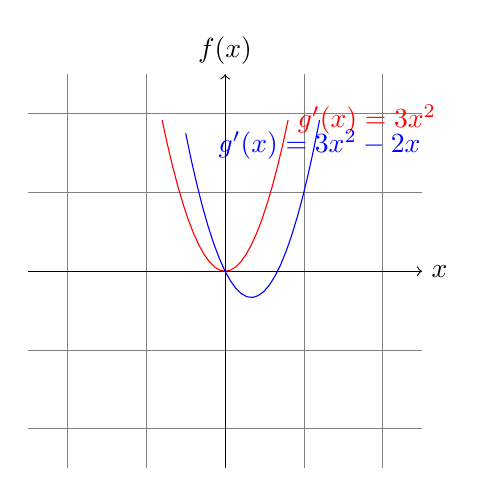
\begin{tikzpicture}
            \draw[very thin,color=gray] (-2.5, -2.5) grid (2.5, 2.5);
            \draw[->] (-2.5,0) -- (2.5,0) node[right] {$x$};
            \draw[->] (0,-2.5) -- (0,2.5) node[above] {$f(x)$};
            \draw[red,domain=-0.8:0.8]	plot (\x, { 3 * \x * \x })   	node[right] {$g'(x) = 3x^2 $};
            \draw[blue,domain=-0.5:1.2]	plot (\x, { 3 * \x * \x - 2 * \x})   	node[below] {$g'(x) = 3x^2 - 2x$};
        \end{tikzpicture}
    \end{minipage}
    \begin{minipage}[b]{0.32\textwidth}
        \centering
        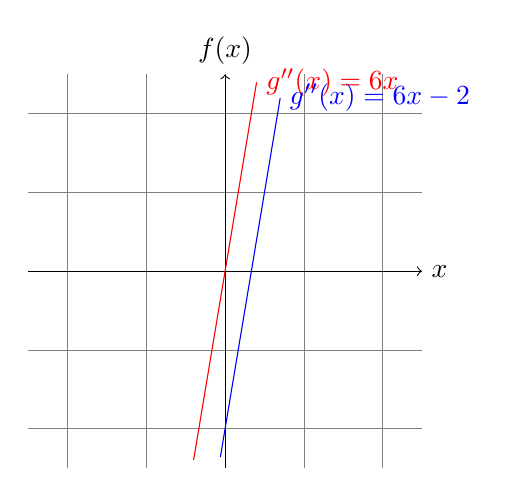
\begin{tikzpicture}
            \draw[very thin,color=gray] (-2.5, -2.5) grid (2.5, 2.5);
            \draw[->] (-2.5,0) -- (2.5,0) node[right] {$x$};
            \draw[->] (0,-2.5) -- (0,2.5) node[above] {$f(x)$};
            \draw[red,domain=-0.4:0.4]	plot (\x, { 6 * \x })   	node[right] {$g''(x) = 6x $};
            \draw[blue,domain=-0.06:0.7]	plot (\x, { 6 * \x - 2 })   	node[right] {$g''(x) = 6x - 2$};
        \end{tikzpicture}
    \end{minipage}
    \caption{Challenges}
\end{figure}


\subsection{Local Minima}
\begin{quotation}
    When the numerical solution of an optimization problem is near the local optimum, the numerical
    solution obtained by the final iteration may only minimize the objective function locally, rather
    than globally, as the gradient of the objective function's solutions approaches or becomes zero.
    \textit{Only some degree of noise might knock the parameter out of the local minimium. In fact,
        this is the one of the beneficial properties of stochastic gradient descent where the natural variation
        of gradients over minibatches is able to dislodge the parameters from loacl minima.}\cite{zhang2020dive}
\end{quotation}
\subsection{Saddle Points}
\begin{quotation}
    We assume that the input of a function is $k$-dimensional vector and its ouput is a scalar,
    so its \textit{Hession matrix} will have \textit{$k$ eigenvalues}. The solution of the function could
    be a local minimum, a local maximum or a saddle point at a position where the function gradient
    is zero:
    \begin{itemize}
        \item When the eigenvalues of the function's Hession matrix at the zero-gradient position 
        are all positive, we have a local minimum for the function.
        \item When the eigenvalues of the function's Hession matrix at the zero-gradient position 
        are all negative, we have a local maximum for the function.
        \item When the eigenvalues of the function's Hession matrix at the zero-gradient position 
        are negative and positive, we have a saddle point for the function.
        \item 同号且至少有一个为0,不确定
    \end{itemize}
    For high-dimensional problem the likehood that at least some of the eigenvalues are negative
    is quite high. This makes sadlle points are more likely then local minima.\cite{zhang2020dive}
\end{quotation}

\subsection{Vanishing gradients}
\begin{quotation}
    Vanishing gradients can cause optimization to stall. Often a reparameterization of the problem
     helps. Good initialization of the parameters can be beneficial, too.\cite{zhang2020dive}
\end{quotation}

\subsection{Gradient Descent}
Using a Taylor expansion we obtain that:
\begin{equation}
    f(x + \epsilon) = f(x) + \epsilon f'(x) + \mathcal{O} (\epsilon^2)
\end{equation}
\par
For small $\epsilon$ moving in \textit{the direction of negative gradient} will decrease $f$. Choose $\epsilon = 
-\eta f'(x), \eta > 0$, then we get:
\begin{equation}
    f(x - \eta f'(x)) = f(x) - \eta f'^2(x) + \mathcal{O} ((\eta f'(x))^2)
\end{equation}
\par Choose $\eta$ samll enough for the higher order terms to become irrelevant. then
\begin{equation}
    f(x - \eta f'(x)) \lessapprox f(x)
\end{equation}
that means, if we use 
\begin{equation}
    x \leftarrow x - \eta f'(x)
\end{equation}
to iterate x, the value of $f(x)$ decline.

\subsection{Adaptive Methods}
Getting the learning rate 'just right' is tricky. What if we could determine $\eta$ automatically or get rid of having to select
a setp size at all? Second order methods that look not only at the value and gradient of the objective but alse at its \textit{curvature}
can help in this case. These methods cannot be applied to deep learning directly due to the computational cost.

\subsubsection{Newton's Method}
当Taylor expansion展开到二阶导数时:
\begin{equation}
    f(\mathbf{x} + \epsilon) = f(\mathbf{x}) + \epsilon^\top \nabla f(\mathbf{x}) + \frac{1}{2} \epsilon^\top H_f \epsilon 
    + \mathcal{O}(\|\epsilon\|^3)
\end{equation}
we define $H_f := \nabla \nabla ^\top f(\mathbf{x})$ to be the \textit{Hession} of $f$. $H$ is a $d \times  d$ matrix and may be
prohibitively large, due to the cost of storing $\mathcal{O}(d^2)$ entries.

\par

After all, the minimum of $f$ statifies $\nabla f(\mathbf{x}) = 0$.  Taking derivatives of above equtaion with regard to $\eta$ and 
ignoring higher order terms we arrive at 
\begin{equation}
   \begin{split}
    \nabla f(\mathbf{x}) + H_f \epsilon = 0 \\
    \mathbf{\epsilon} = -H_f^{-1} \nabla f(\mathbf{x})
   \end{split}
\end{equation}

then, $\epsilon = -\eta \nabla f(\mathbf{x})$, we get
\begin{equation}
    \begin{split}
        \mathbf{\eta} = -H_f^{-1}
    \end{split}
\end{equation}

For $f(x) = (x-2)(x-4) = x^2 - 6x + 8, f'(x) = 2x - 6, f''(x) = 2$, then
\begin{equation}
    \epsilon = -f''(0)^{-1} f'(0) = -\frac{1}{2} \times -6 = 3 
\end{equation}

\subsubsection{Hessian}
Hession 矩阵是是对称的,可以表示为一组特征值和一组特征向量的正交基底,在特定方向上$g$上的二阶导数为$g^\top H g$,当$g$为特征向量时,这个二阶导数就是
对应的特征值。最大特征值确定最大二阶导数,最小特征值确定最小导数。\par
在$g$方向上的learning rate为
\begin{equation}
    \eta_g = \frac{1}{g^\top H_f g}
\end{equation}
最差的情况下,$g$与$H$最大的特征值$\lambda_{max}$对应的特征向量对齐,此时的最优步长为$\frac{1}{\lambda_{max}}$,当要最小化的目标函数能用二次函数
很好近似的情况下,Hession的特征值决定了学习率的量级。

\subsection{Stochastic Gradient Descent}
\subsubsection{Dynamic Learning rate}

\begin{equation}
    \begin{aligned}
        \eta(t) &= \eta_i \text{ if } t_i \leq  t \leq t_{i+1} & & piecewise constant\\
        \eta(t) &= \eta_0 e^{-\lambda t} & & exponential\\
        \eta(t) &= \eta_0 (\beta t + 1) ^{-\alpha} && polynomial
    \end{aligned}
\end{equation}
In the case of convex optimization there are a number of proofs which show that this rate is well behaved.

\subsection{Minibatch Stochastic Gradient Descent}